\documentclass[conference]{IEEEtran}
\usepackage{amsmath,amssymb}
\usepackage{booktabs}
\usepackage{array}
\usepackage{graphicx}
\usepackage{cite}
\usepackage{url}
\usepackage[hidelinks,breaklinks=true]{hyperref}
\title{An Experimental and Theoretical Analysis of Adam: Convergence, Computational Complexity, and Comparison with SGD-Momentum and AMSGrad}
\author{\IEEEauthorblockN{Dario Pomasqui}\IEEEauthorblockA{School of Mathematical and Computational Sciences\\Yachay Tech University\\ECMC1018 Analysis of Algorithms}}
\begin{document}
\maketitle
\begin{abstract}
This preliminary study examines Adam (Adaptive Moment Estimation) as a vector optimization algorithm through a C++17 implementation and deterministic test objectives. We compare Adam with SGD using momentum and AMSGrad on quadratic, Rosenbrock, Rastrigin, and a periodic-gradient counterexample associated with prior convergence analysis. The optimizer update has linear time and auxiliary memory in the parameter dimension when the gradient is available. In the tested settings, all methods approached the quadratic and Rosenbrock minima under their declared stopping tolerances; on Rastrigin, small gradient norms occurred at non-global local minima. In the periodic-gradient example, Adam and AMSGrad showed distinct behavior after 300,000 updates. These observations are configuration-specific and do not establish general superiority or convergence guarantees. The study documents equations, implementation checks, experimental limitations, and reproducible commands.
\end{abstract}
\begin{IEEEkeywords}
Adam, stochastic optimization, AMSGrad, momentum, algorithm analysis, C++
\end{IEEEkeywords}
\section{Introduction}
First-order optimization methods repeatedly use objective gradients to update a parameter vector. Adam combines exponentially weighted gradient and squared-gradient statistics to produce coordinate-wise adaptive steps \cite{kingma}. It is widely used, but its empirical effectiveness does not imply universal convergence. Reddi et al. exhibit settings where Adam's adaptive learning rates can fail and propose AMSGrad \cite{reddi}.

This project asks: how does Adam behave on representative objective landscapes, and how do its convergence observations and computational costs compare with momentum SGD and AMSGrad? The scope is deliberately a small, deterministic C++ benchmark. It does not claim results for neural networks or stochastic minibatch training; stochastic optimization in machine learning has distinct sampling and noise considerations \cite{bottou}.
\section{Background}
Adam maintains first- and second-moment estimates with bias correction \cite{kingma}. Reddi et al. identify a non-convergence issue in some settings and propose AMSGrad, which keeps a coordinate-wise maximum of second moments \cite{reddi}. Momentum SGD uses accumulated velocity; the heavy-ball method is associated with Polyak \cite{polyak}.
\section{Problem and Algorithms}

\subsection{Motivation for Adaptive Learning Rates}
Gradient descent with a fixed scalar step size applies the same learning rate to every coordinate of the parameter vector. When coordinates have substantially different gradient magnitudes---for example, a feature that appears rarely in a dataset versus one that appears frequently---a single rate must be small enough not to overshoot the sensitive coordinate while still being large enough to make progress on the other. This is the core scaling problem that adaptive methods address. Adam addresses it by replacing a cumulative sum of squared gradients with an exponential moving average controlled by $\beta_2$, so the effective denominator tracks a finite historical window rather than the entire past \cite{kingma}.

\subsection{Adam: Derivation and Update Rule}
For a differentiable objective $f:\mathbb{R}^d\to\mathbb{R}$, the deterministic experiments use the full gradient $g_t=\nabla f(\theta_t)$. Adam maintains two exponentially weighted statistics. The first moment $m_t$ approximates the mean of recent gradients, providing directional momentum:
\begin{equation}
  m_t = \beta_1 m_{t-1} + (1-\beta_1)\,g_t.
\end{equation}
The second moment $v_t$ tracks an exponentially weighted average of squared gradients, providing a coordinate-wise estimate of their recent magnitude:
\begin{equation}
  v_t = \beta_2 v_{t-1} + (1-\beta_2)\,g_t^2.
\end{equation}
Both are initialized at zero: $m_0 = v_0 = 0$.

\subsection{Bias Correction}
Because the moments are initialized at zero, their early values are biased toward zero regardless of the gradient signal. To see this, expanding the recurrence for $m_t$ gives:
\begin{equation}
  m_t = (1-\beta_1)\sum_{i=1}^{t}\beta_1^{t-i}\,g_i.
\end{equation}
Under the assumption that $\mathbb{E}[g_t]=\mu_g$ for all $t$:
\begin{equation}
  \mathbb{E}[m_t] = \mu_g\left(1 - \beta_1^t\right).
\end{equation}
Dividing by $(1-\beta_1^t)$ removes the initialization bias in expectation:
\begin{equation}
  \hat{m}_t = \frac{m_t}{1-\beta_1^t}.
\end{equation}
The analogous correction for the second moment is:
\begin{equation}
  \hat{v}_t = \frac{v_t}{1-\beta_2^t}.
\end{equation}
Both correction factors approach 1 as $t\to\infty$, so the correction becomes negligible in later iterations and the algorithm recovers the standard exponential moving average. The bias correction is therefore most significant in early iterations, as confirmed by the first-step unit checks in the test suite.

\subsection{Parameter Update and Epsilon Placement}
The full update, applied element-wise across all $d$ coordinates, is:
\begin{align}
  \hat{m}_t &= m_t/(1-\beta_1^t), &\hat{v}_t &= v_t/(1-\beta_2^t),\\
  \theta_{t+1} &= \theta_t - \alpha\,\hat{m}_t\,/\,(\sqrt{\hat{v}_t}+\epsilon).
\end{align}
The scalar $\epsilon > 0$ prevents division by zero and stabilizes coordinates where the second moment is near zero---typically when the gradient has been consistently close to zero along that direction. In this implementation $\epsilon$ is added \emph{after} the square root, matching the convention in Kingma and Ba \cite{kingma}. Placing $\epsilon$ inside the root would yield a different effective step in small-variance coordinates and is not the form used here.

\subsection{Role of Hyperparameters}
Default values are $\alpha=0.01$, $\beta_1=0.9$, $\beta_2=0.999$, $\epsilon=10^{-8}$, unless a specific experiment declares overrides.
\begin{itemize}
  \item $\alpha$ (learning rate): scales the magnitude of every update. A too-large value can cause oscillation or overshoot; a too-small value slows convergence. The Rosenbrock sweep in Table~\ref{tab:lr} shows how iteration count varies across a grid of tested rates.
  \item $\beta_1$ (first-moment decay): controls how far back the directional average reaches. A value near 1 averages over a long history; a value near 0 is closer to the current gradient. At 0.9 the effective window is approximately $1/(1-0.9)=10$ recent steps.
  \item $\beta_2$ (second-moment decay): analogously controls the magnitude memory. At 0.999 the effective window is approximately 1000 steps, making the denominator a slowly adapting scale. In the Reddi example $\beta_2=0.99$ is used to increase responsiveness of the denominator to the periodic large gradient event.
  \item $\epsilon$: a numerical safety term. In practice it also softens the adaptive scaling---when $\hat{v}_t$ is small but nonzero, $\epsilon$ limits how large the effective step can grow relative to the recent gradient scale in that coordinate.
\end{itemize}

\subsection{Comparison Methods}
Momentum SGD follows $u_t=\beta u_{t-1}+g_t$ and $\theta_{t+1}=\theta_t-\alpha u_t$. It accumulates gradient direction but does not apply coordinate-wise magnitude scaling. The implementation stores $\alpha u_t$ as its velocity, with zero initialization. Its experiment parameters are declared in the runner.

AMSGrad follows the uncorrected-moment variant in Reddi et al. \cite{reddi}: $m_t=\beta_1 m_{t-1}+(1-\beta_1)g_t$, $v_t=\beta_2 v_{t-1}+(1-\beta_2)g_t^2$, $v_t^{\max}=\max(v_{t-1}^{\max},v_t)$ element-wise, and $\theta_{t+1}=\theta_t-\alpha m_t/(\sqrt{v_t^{\max}}+\epsilon)$. It does not use Adam's bias correction in this implementation. The nondecreasing denominator is the key structural difference from Adam: once a large gradient event inflates $v_t^{\max}$, subsequent steps in that coordinate cannot grow as fast as Adam's exponentially decaying $\hat{v}_t$ would allow.

\section{Theoretical Analysis}

\subsection{Per-Step Computational Complexity}
With the gradient supplied, each optimizer update loops over $d$ coordinates and performs a constant number of arithmetic operations per coordinate:
\begin{itemize}
  \item Momentum: one weighted accumulation and one subtraction per coordinate $\Rightarrow$ $O(d)$ time, $O(d)$ state (one velocity vector).
  \item Adam: two moment accumulations, two bias-correction divisions (shared scalar factors), one square root and denominator, and one parameter update per coordinate $\Rightarrow$ $O(d)$ time, $O(d)$ state (two vectors $m$ and $v$).
  \item AMSGrad: same as Adam plus one element-wise maximum comparison $\Rightarrow$ $O(d)$ time, $O(d)$ state (three vectors $m$, $v$, and $v^{\max}$).
\end{itemize}
Gradient-evaluation cost is additional to the optimizer update. For the separable quadratic and Rastrigin objectives, gradient evaluation costs $O(d)$. For the fixed two-dimensional Rosenbrock objective used here, gradient evaluation costs $O(1)$. These objective-specific costs are separate from the $O(d)$ optimizer update bound, which applies when the gradient is available \cite{nocedal}.

\subsection{Convergence Considerations}
Kingma and Ba derive an $O(\sqrt{T})$ regret bound under the assumptions of their analysis for online convex optimization \cite{kingma}. Reddi et al. later identify a limitation in that analysis and present a simple convex setting in which Adam does not converge to the optimum. They propose AMSGrad to address this failure mode \cite{reddi}. These theoretical results are conditional and do not establish a universal convergence guarantee for every configuration of either optimizer.

In the deterministic experiments studied here, convergence guarantees require assumptions (convexity, Lipschitz gradients) that are not verified for every objective. The quadratic objective is strongly convex and provides the clearest setting; Rosenbrock is smooth but nonconvex; Rastrigin is nonconvex with multiple local minima. All convergence guarantees are therefore conditional and should not be extrapolated beyond the stated experimental conditions. Recent analyses continue to refine the conditions and rates under which Adam converges, including stochastic quadratic settings \cite{dereich}. The observations reported below are measured results under specific configurations, not proofs of global convergence.
\section{Implementation and Experimental Setup}
The C++17 implementation uses the C++ standard vector type and CMake. It validates learning rates, moment parameters, vector sizes and finite values; invalid inputs throw exceptions rather than silently skipping an update. The test executable checks analytic gradients at known points, first-step updates, reset behavior, and invalid inputs. Experiments use the same start, maximum iteration limit and gradient tolerance for methods within a given objective. Learning rates vary between algorithms and were not tuned with an equal search budget, so iteration counts describe the selected configurations rather than an intrinsic ranking.

The test functions are $f(x)=\sum_i x_i^2$ (2D and 10D), Rosenbrock $f(x,y)=(1-x)^2+100(y-x^2)^2$ with minimum $(1,1)$, and Rastrigin $f(x)=10d+\sum_i[x_i^2-10\cos(2\pi x_i)]$ with global minimum at the origin. A separate periodic-gradient experiment follows the construction used by Reddi et al. and projects the scalar iterate to $[-1,1]$. CSV files record iteration, objective, gradient norm, distance to the known optimum, and coordinates where applicable. Wall-clock times are one-run observations and are not robust benchmark estimates.
\section{Results and Discussion}
For the quadratic 2D case from $(5,-3)$, the gradient tolerance was $10^{-8}$. The observed iteration counts were 2619 for Adam, 339 for momentum SGD and 1639 for AMSGrad. For Rosenbrock from $(-1.5,2)$ with tolerance $10^{-6}$, they were 4443, 3118 and 16057, respectively. All reached the stated gradient criterion in these runs.

On 2D Rastrigin from $(2.5,2.5)$, all methods reached gradient norm below $10^{-6}$, yet Adam and AMSGrad ended at objective approximately 7.96 and momentum SGD at approximately 1.99. This demonstrates that a small gradient norm is not evidence of reaching the global minimum on a multimodal objective. It does not establish comparative global-search ability.

In the periodic-gradient run after 300,000 updates, Adam ended near $x=0.9454$ and AMSGrad near $x=-0.9982$, while the target is $-1$. This is consistent with the purpose of the constructed example, but this finite run is a reproduction under the implementation's stated hyperparameters, not a general theorem. The Rosenbrock learning-rate sweep also showed sensitivity: with maximum 20,000 iterations, $\alpha=0.0001$ did not meet tolerance, while $\alpha=0.1$ did so in 1463 steps. Intermediate values and raw trajectories are provided in CSV.

Elapsed-time summary values were collected once per run and are sensitive to compilation, process scheduling and machine state. We therefore do not use them to make general speed claims. The optimizer's asymptotic update costs remain linear in $d$ under the stated assumption that gradients are already available.
\subsection{Research Questions and Hypotheses}
The project examines three questions. RQ1 compares observed trajectories and stopping iterations on a quadratic and the curved Rosenbrock valley, a classic nonlinear test problem introduced in early numerical optimization work \cite{rosenbrock}. RQ2 studies Adam's learning-rate sensitivity on Rosenbrock from one fixed initial point. RQ3 checks whether the Reddi periodic-gradient construction produces different finite-run behavior for Adam and AMSGrad. The hypotheses were that the simple quadratic would be manageable for each method with suitable rates, the Rosenbrock valley would expose sensitivity to step scale, and the multimodal Rastrigin function would make initialization relevant. Benchmark function surveys emphasize that test landscapes capture different properties and cannot alone support broad optimizer rankings \cite{benchmark}. These are motivations; outcomes below are measured results.
\subsection{Objective Derivatives and Checks}
For $f(\mathbf{x})=\sum_i x_i^2$, $\nabla f=2\mathbf{x}$ and the global minimum is the origin. Rosenbrock's derivatives are $\partial f/\partial x=-2(1-x)-400x(y-x^2)$ and $\partial f/\partial y=200(y-x^2)$; both vanish at $(1,1)$, where $f=0$. Rastrigin has coordinate derivative $2x_i+20\pi\sin(2\pi x_i)$ and global minimum zero at the origin. Unit checks compare objective and derivatives at known points. Such checks catch implementation mistakes but do not prove correctness for all floating-point inputs.

The Reddi case supplies a prescribed gradient sequence rather than evaluating the derivative of a fixed scalar objective: $C=101$, $g_t=C$ when $t\bmod C=1$, otherwise $g_t=-1$. The scalar iterate is projected onto $[-1,1]$. Consequently, the plotted x trajectory and distance to target are interpretable, but an objective-loss column is not defined for this experiment.
\subsection{Implementation Details}
The optimizers store state in the C++ standard vector type, initialize moments to zero on the first call, and require the reset method between independent runs. Adam increments $t$ before bias correction. Its epsilon is added outside the square root. Parameters and gradients must have matching dimensions and finite entries; learning rate, beta values, epsilon and momentum are validated. A non-finite input or update raises an exception instead of silently skipping a coordinate. An optimizer state cannot change dimension without reset.

The runner evaluates $f(\theta_t)$ and $g_t$, logs metrics for the current point, checks the stopping condition, then applies the step that yields $\theta_{t+1}$. Thus CSV row $t$ records the pre-update state. Main comparison tolerances are $10^{-8}$ for quadratics and $10^{-6}$ for Rosenbrock and Rastrigin. Reddi uses a fixed 300,000-update budget. The Momentum implementation stores $\alpha u_t$ as its velocity, equivalent to $u_t=\beta u_{t-1}+g_t$ with constant $\alpha$ and zero state. AMSGrad uses uncorrected $m_t$, $v_t$, and running maximum $v_t^{\max}$, following the variant described in Reddi et al.; it is not Adam with a corrected numerator.
\subsection{Experimental Protocol and Hyperparameters}
The deterministic experiments use analytic full gradients, with no random data or sampling seed. The 2D quadratic starts at $(5,-3)$, the 10D quadratic uses the fixed vector in the main runner source, Rosenbrock starts at $(-1.5,2)$, and Rastrigin starts at $(2.5,2.5)$. For each objective, the methods share the start, maximum iteration count, stopping tolerance and objective implementation. Rates are declared per method in the runner but were not selected via an equal-budget search; iteration counts therefore compare these configurations, not an intrinsic ordering of algorithms.

For quadratic tests the rates are $0.01$ for Adam, Momentum and AMSGrad, with Momentum coefficient $0.9$. For Rosenbrock, Adam and AMSGrad use $0.01$ while Momentum uses $0.001$ and coefficient $0.9$. For Rastrigin, Adam and AMSGrad use $0.05$, while Momentum uses $0.005$ and coefficient $0.9$. Adam and AMSGrad use $\beta_1=0.9$, $\beta_2=0.999$, $\epsilon=10^{-8}$ except the Reddi example, which uses $\beta_2=0.99$. The Adam Rosenbrock sweep tests $\alpha\in\{0.0001,0.0005,0.001,0.005,0.01,0.05,0.1\}$ with other settings fixed and a 20,000-step cap.

CSV records iteration, objective, gradient norm, distance to known optimum and coordinates. The summary records final metrics, iteration count, one-run elapsed milliseconds, convergence status, stopping reason and hyperparameters. Trajectory files use iteration intervals specified in the runner. Repeated wall-clock measurements are not included, so execution-time differences are descriptive only.
\subsection{Detailed Results}
Table~\ref{tab:results} summarizes the main deterministic runs. All quadratic runs attained the $10^{-8}$ gradient-norm threshold. On 2D the observed counts were 2619, 339 and 1639 for Adam, Momentum and AMSGrad; on 10D they were 2639, 362 and 1666. Final distances in the 2D case were about $5\times10^{-9}$. Similar iteration counts between 2D and 10D are consistent with the separable isotropic objective, but the tested dimension range is too small to establish a scaling law empirically.

On Rosenbrock, all methods met the $10^{-6}$ gradient criterion: Adam used 4443 steps, Momentum 3118 and AMSGrad 16057. Their final objective values were approximately $10^{-12}$ and distances from $(1,1)$ a few $10^{-6}$. These endpoints indicate successful minimization for this start and configuration. The lower Momentum count cannot be generalized because the rates were selected separately.

On Rastrigin all three methods met the gradient threshold, but their final objectives were not the global minimum zero. Adam and AMSGrad reached about 7.96 at distance 2.81, while Momentum reached about 1.99 at distance 1.41. This is a concrete reason to report objective and distance in addition to gradient norm: a small gradient can mark a non-global stationary point in a multimodal objective.

In the 300,000-step periodic-gradient construction Adam ended at approximately $0.9454$ and AMSGrad at approximately $-0.9982$, with target $-1$. The result shows contrasting finite-run behavior in this construction and agrees qualitatively with the motivation for AMSGrad. It does not prove universal convergence of AMSGrad or universal failure of Adam.

The Adam learning-rate sweep on Rosenbrock did not meet tolerance for $\alpha=10^{-4}$ within 20,000 steps (final gradient norm approximately 2.41). For the remaining tested rates, observed counts were 15919 ($0.0005$), 11647 ($0.001$), 6059 ($0.005$), 4443 ($0.01$), 2022 ($0.05$) and 1463 ($0.1$). In this finite range, increasing the tested rate reduced the steps to the criterion. This pattern may change outside the tested range, with another function or initial point.
\begin{table}[t]
\caption{Observed iterations to gradient tolerance}
\label{tab:results}
\centering
\small
\begin{tabular}{llrrr}
\toprule
Objective & Tolerance & Adam & Momentum & AMSGrad\\
\midrule
Quadratic 2D & $10^{-8}$ & 2619 & 339 & 1639\\
Quadratic 10D & $10^{-8}$ & 2639 & 362 & 1666\\
Rosenbrock & $10^{-6}$ & 4443 & 3118 & 16057\\
Rastrigin & $10^{-6}$ & 318 & 304 & 291\\
\bottomrule
\end{tabular}
\end{table}
\begin{figure}[t]
\centering
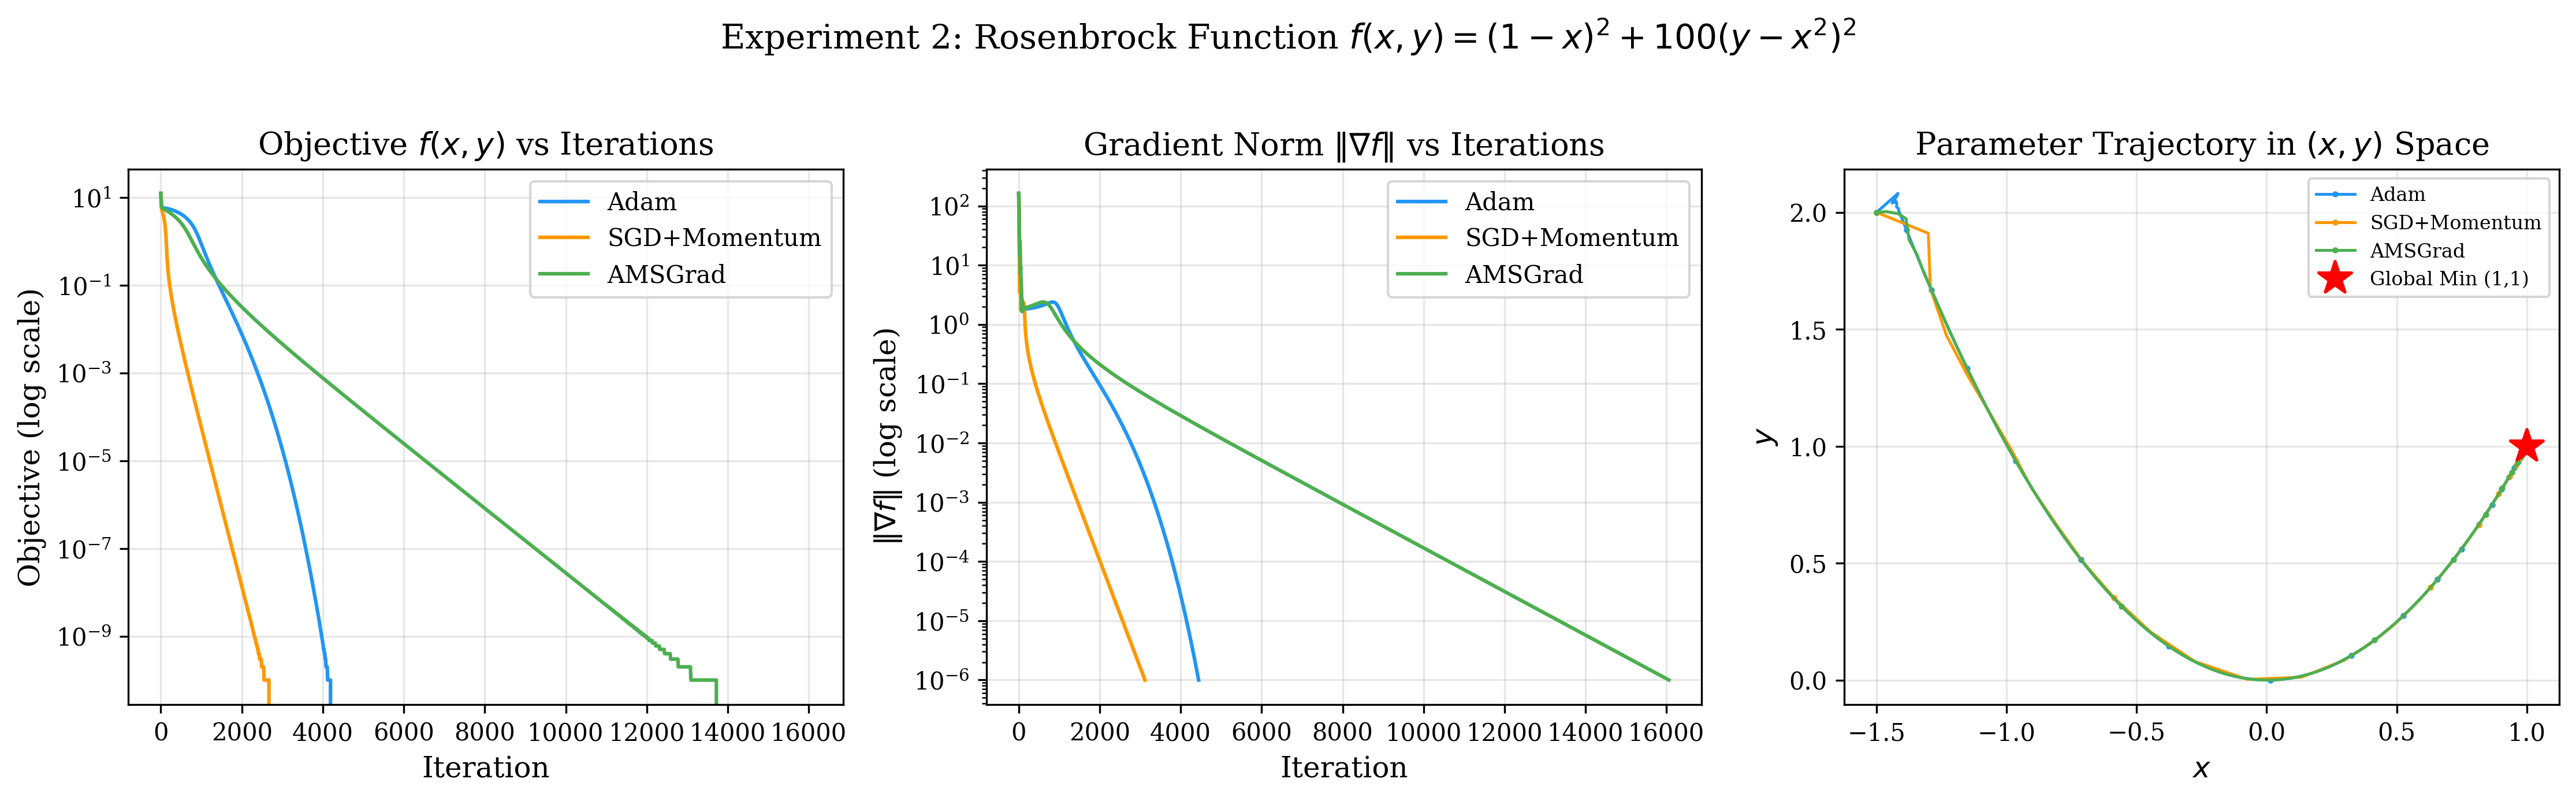
\includegraphics[width=0.48\textwidth]{figures/rosenbrock_comparison.png}
\caption{Rosenbrock objectives, gradient norms and parameter trajectories generated from the recorded CSV files.}
\label{fig:rosenbrock}
\end{figure}
\begin{figure}[t]
\centering
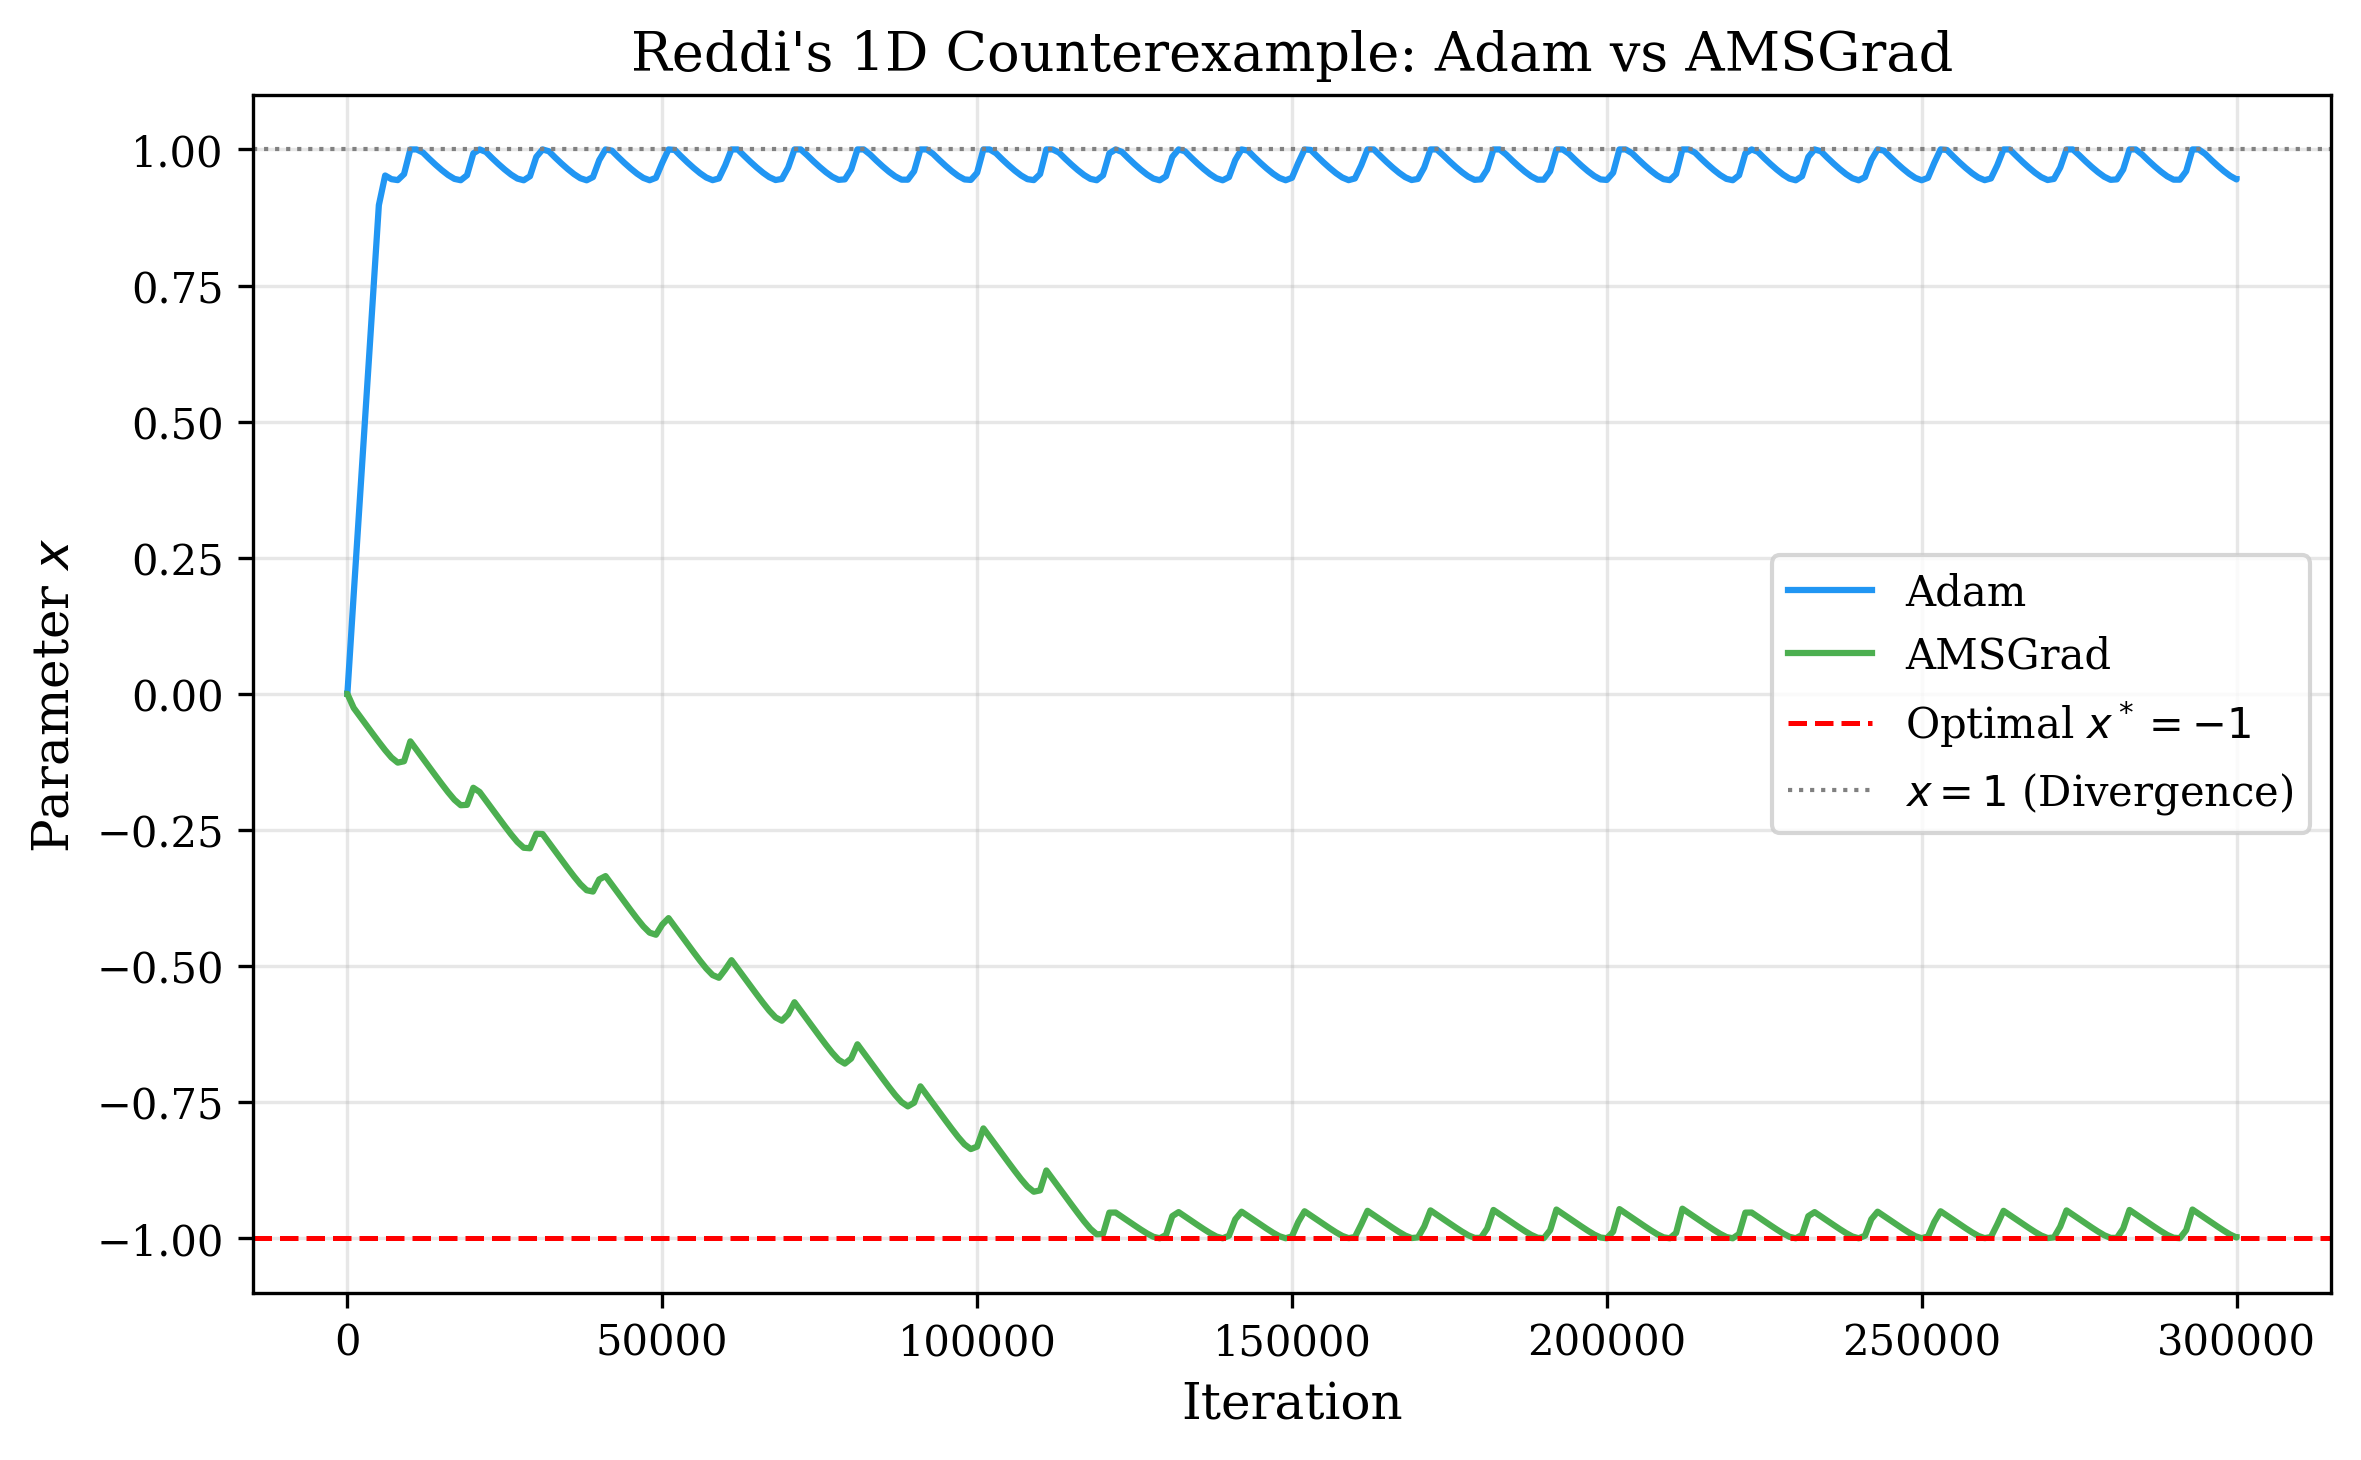
\includegraphics[width=0.48\textwidth]{figures/reddi_counterexample.png}
\caption{Finite-run scalar iterates in the periodic-gradient construction.}
\label{fig:reddi}
\end{figure}
Figure~\ref{fig:rosenbrock} visualizes the narrow curved valley and the different paths taken under the declared rates. Figure~\ref{fig:reddi} shows that the contrast in the constructed gradient sequence accumulates over many updates. Both figures are generated by the plotting script from the current CSV files.
\subsection{Complexity Interpretation}
For dimension $d$, Adam performs a constant number of coordinate-wise operations, including moment updates, bias correction, square root and parameter update, yielding $O(d)$ optimizer time per iteration. It keeps two optimizer state vectors ($m,v$), or $O(d)$ auxiliary memory. Momentum has one state vector and $O(d)$ memory; AMSGrad stores $m,v,v^{\max}$ and also uses $O(d)$. These counts exclude the parameter vector, gradient vector and objective data/model storage. Gradient computation has a separate cost dependent on the objective. Asymptotic per-step work does not imply fewer iterations or faster convergence. Empirical times from one run do not replace asymptotic analysis.
\subsection{Threats to Validity}
The tests are low-dimensional, analytic, deterministic, and use a single start per function. They omit stochastic minibatches, data loading, neural network models and high-dimensional memory pressure. Hyperparameter settings are stated but not tuned under a common budget, so iteration counts are not a controlled estimate of an optimizer's best performance. Gradient norm can be misleading about global optimality, as Rastrigin shows. Runtime measurements are from one Windows environment and one run per case. The Reddi example is a particular gradient sequence and projection, not representative of every training problem. Accordingly, findings are limited to the code, data, initial points, stopping rules and rates described here.
\subsection{Reproducibility and Validation}
The implementation uses C++17, CMake 3.29, MinGW g++ 13.2 and Ninja on Windows. Run from the project directory: configure with the CMake Release configure command, build with the clean build command, run checks with the CTest command, execute the generated executable, then generate plots with the plotting script. Python is only used for plotting; all optimizers and objectives are C++.

CTest checks the quadratic value and gradient at $(2,-3)$, the known Rosenbrock/Rastrigin minima, first updates for each method, reset, invalid hyperparameters, dimension changes and non-finite gradients. The clean build and the test suite passed before this report update. CSV and plots were regenerated in the current run. The summary timing column is retained for transparency but should be interpreted cautiously.
\section{Algorithm and Measurement Analysis}
Adam's first moment is an exponential moving average, so it carries directional information across iterations. If successive gradients point in similar directions, this average preserves a substantial update; if they alternate, partial cancellation can reduce it. The second moment tracks recent squared magnitude and is nonnegative coordinate-wise. Dividing by its square root normalizes each coordinate relative to recent gradient scale. Bias correction matters most early because zero initialization depresses the raw averages: at $t=1$, the corrected values recover the current gradient and squared gradient when $\beta_1,\beta_2<1$. This first-step property is directly checked in the unit tests.

The adaptive denominator can produce a coordinate-wise effective step scale. That mechanism is useful for analyzing differently scaled coordinates, but it also means the update depends on gradient history and not solely on the current objective slope. Adam is therefore not equivalent to applying a fixed scalar learning rate to a smoothed gradient. The chosen $\epsilon$ placement also matters numerically: adding it after the square root is the convention encoded by this implementation, and formulas that put epsilon inside the root would define a different update in small-variance coordinates.

The deterministic tests provide full exact gradients. In practical stochastic optimization, $g_t$ may be a noisy minibatch estimate. The moving averages then track a stochastic sequence and the interpretation of observed loss curves changes. No such sampling noise is present in these experiments, so the results isolate optimizer recurrence and objective geometry rather than a full machine-learning training pipeline.
\subsection{Why the Comparison Methods Are Appropriate}
Momentum SGD is a useful baseline because it retains directional memory but does not divide by a coordinate-wise second-moment estimate. The comparison can therefore show trajectories where both methods exploit accumulated direction, while their step scaling differs. To keep the selected variant explicit, the implementation uses the heavy-ball recurrence with constant coefficient $\beta$ and learning rate applied to the accumulated velocity. It does not implement Nesterov momentum, dampening, or decoupled weight decay.

AMSGrad is included because the convergence limitation studied by Reddi et al. is directly related to Adam's adaptive second-moment history. Its running maximum is nondecreasing per coordinate, preventing the denominator's stored second-moment scale from decreasing in the same manner as Adam's exponential average. This modification changes the effective steps and can make them more conservative. The current experiments demonstrate a difference on the constructed periodic-gradient sequence; they do not test all assumptions of the paper's theorem, nor do they imply AMSGrad is best on arbitrary objectives.

A fair empirical comparison requires more than identical initial points. Hyperparameter selection budget, stopping criteria, objective evaluation cost, repetitions and hardware all affect interpretation. We match starts, caps and tolerances within each objective, and make the unequal rates visible. We do not claim that one method is intrinsically faster based on these chosen rates.
\subsection{Additional Results: Learning-Rate Sweep}
Table~\ref{tab:lr} reports the seven tested rates. The lowest rate did not reach tolerance before the 20,000-step cap; the remaining six did. Objective values and final gradient norms are in the learning-rate sweep CSV, and the corresponding loss and trajectory views are in the generated learning-rate figures. The apparent trend across this finite list should be read narrowly: rates above 0.1 and other starting points were not evaluated, and the sweep contains no repeats because the optimization path is deterministic.
\begin{table}[t]
\caption{Adam learning-rate sweep on Rosenbrock; cap 20,000, tolerance $10^{-6}$}
\label{tab:lr}
\centering
\begin{tabular}{rrrl}
\toprule
$\alpha$ & Iterations & Final objective & Status\\
\midrule
0.0001 & 20000 & 2.9106 & cap\\
0.0005 & 15919 & $1.0955\times10^{-12}$ & tolerance\\
0.0010 & 11647 & $9.9576\times10^{-13}$ & tolerance\\
0.0050 & 6059 & $9.5550\times10^{-13}$ & tolerance\\
0.0100 & 4443 & $9.6432\times10^{-13}$ & tolerance\\
0.0500 & 2022 & $9.6279\times10^{-13}$ & tolerance\\
0.1000 & 1463 & $9.4450\times10^{-13}$ & tolerance\\
\bottomrule
\end{tabular}
\end{table}
\subsection{Memory and Operation Accounting}
For each coordinate, Adam stores two persistent state values, $m_i$ and $v_i$. A step updates both, computes two bias-correction divisions using scalar correction factors shared across coordinates, evaluates a square root and denominator, and updates $\theta_i$. Thus the number of arithmetic operations grows linearly with $d$. AMSGrad stores $m_i$, $v_i$, and $v_i^{\max}$ and adds a maximum comparison per coordinate; its asymptotic time and state remain $O(d)$. Momentum stores one velocity value and performs a constant number of operations per coordinate, also $O(d)$ time and memory. The exact operation constants differ, but asymptotic notation suppresses them.

This state accounting treats optimizer auxiliary memory as the persistent state required by the recurrence. The parameter and gradient arrays are required by all methods and should be reported separately in a detailed implementation-level memory measurement. The experiment runner also allocates temporary vectors and output buffers; these are not optimizer state. For a model with $d$ parameters, the number of stored state scalars is proportional to $d$, but total program memory can be dominated by model data or gradient evaluation.

The experiment's wall-clock times combine gradient calculation, optimizer update, logging and loop overhead. Since the objectives are tiny and CSV logging is active, these timings are not a clean measurement of the update kernel. A benchmark designed to estimate optimizer-only runtime would need to separate gradient and output costs, warm up, repeat runs, and report dispersion. The current report accordingly treats time as an exploratory logged metric rather than a conclusion.
\section{Interpretation of Results}
For RQ1, all methods reached the stopping rule on the quadratic and Rosenbrock cases, with iteration counts depending on selected rates; on the tested Rosenbrock setup, Momentum had the smallest count and AMSGrad the largest. Since settings are not tuned equally, the defensible conclusion is that the tested trajectories differ, not that Momentum dominates on curved valleys. On Rastrigin, methods stopped at different local stationary points, demonstrating the role of multimodality and the limits of a gradient-only stopping rule.

For RQ2, the tested Rosenbrock sweep shows a strong change in steps-to-tolerance over $10^{-4}$ to $10^{-1}$. The run at $10^{-4}$ exhausted its budget, while the largest tested rate reached tolerance in 1,463 updates. This answers the question for the finite tested interval; it does not locate a globally optimal rate.

For RQ3, the finite Reddi sequence ended near 0.945 for Adam and -0.998 for AMSGrad against target -1. This confirms a substantial observed difference for this sequence, initialization, projection and hyperparameters. The experiment is illustrative and does not replace the convergence analysis or prove a universal property.
\subsection{Trajectory-Level Analysis of the Main Objectives}
The endpoint table answers whether the stopping rule was reached, but it hides how an optimizer approached the solution. The trajectory files therefore provide the primary evidence for describing progress. For the quadratic objective, the loss is the squared Euclidean norm and the gradient norm is exactly twice the distance to the minimizer. A log-scale plot of either quantity should consequently show a close relationship. The 2D start has norm $\sqrt{34}$ and initial gradient norm $2\sqrt{34}\approx11.66$; the 10D start has squared norm 110 and initial gradient norm $2\sqrt{110}\approx20.98$. These values agree with the first CSV records. At the stopping threshold $10^{-8}$, the corresponding distance threshold is $5\times10^{-9}$, which is also consistent with the recorded endpoints. This algebraic relation provides an independent check that the implementation, metric calculation and known optimum agree for this objective.

For the 2D case, Adam's adaptive statistics lead to coordinate updates that initially have similar magnitudes even though the two coordinates start at 5 and -3. Momentum instead scales each gradient by the same learning rate and carries its velocity; its selected learning rate is also 0.01 on this experiment. AMSGrad maintains a nondecreasing maximum of the second moment, which changes its denominator history compared with Adam. The observed differences in iteration counts therefore arise from their recurrences and state histories under the configured rates. Since this quadratic is isotropic and separable, it does not test how the methods behave under ill-conditioning or different curvature by direction.

The 10D extension uses the fixed start $(5,-3,2,-4,1,-2,3,-1,4,-5)$, with the same objective summed independently over coordinates. The number of iterations is similar to the 2D experiment for each method, but this is not evidence that optimizer cost is independent of dimension. The iteration criterion is based on the Euclidean norm, the objective has identical curvature in every coordinate, and the dimension range is only two to ten. The per-step operation count still grows proportionally to the number of coordinates, as established by the algorithm analysis.

Rosenbrock is more informative about coupled curvature. The valley follows approximately $y=x^2$ and narrows as the iterate approaches $(1,1)$. The Hessian has substantially different curvature directions near the minimum, and progress often combines motion along the valley with correction toward it. The objective plot and parameter trajectory show that reaching a small loss and a small gradient are related but distinct criteria. The stopping rule is based only on gradient norm; the known optimum distance is retained as an additional diagnostic. All three algorithms ended within a few millionths of the known minimizer for this run, but they required very different numbers of evaluations. The momentum learning rate is one tenth of the Adam and AMSGrad rates, which makes the iteration comparison descriptive of these tuned-by-hand configurations rather than a controlled algorithm-only effect.

Rastrigin contributes nonconvexity and multiple local minima. Its oscillatory cosine terms create repeated basins, so a local stationary point can have a small gradient without being the global solution. The recorded final objectives are positive and the distances to the origin are nonzero, despite the gradient tolerance being satisfied. Momentum's endpoint has lower objective than the endpoints of Adam and AMSGrad for this start, but this single trajectory does not demonstrate stronger global search. Testing additional initial points and reporting the distribution of reached basins would be required for such a claim.
\subsection{Detailed Review of the Learning-Rate Experiment}
The learning-rate sweep holds the Rosenbrock start, moment parameters, epsilon, stopping norm and update budget fixed while changing only Adam's learning rate. This isolates the effect of the scalar rate within one algorithm more directly than the three-method comparisons. At $10^{-4}$ the algorithm makes progress but the norm remains approximately 2.41 at the 20,000-update cap. This is a budget-limited run, not a divergent run: parameters remain finite and the objective is about 2.91. It should be described as "did not reach tolerance within the cap," not "failed to converge" without qualification.

From $5\times10^{-4}$ through $10^{-1}$, each tested run reaches the configured norm threshold. The iteration count decreases across these six tested values, from 15,919 to 1,463. Final losses cluster near $10^{-12}$ and final distances are around $2.2\times10^{-6}$. This similarity of endpoint quality suggests that, for this particular start and finite grid, the main observed rate effect is the number of updates required to reach the selected tolerance. It does not show that the objective trajectories are uniformly monotone or that larger learning rates always improve optimization. The chosen set stops at 0.1, and rate behavior can change abruptly beyond the range or on another objective.

The sweep CSV and figure retain wall-clock measurements, but the timing field is influenced by iteration count, timer resolution, CSV output, operating-system scheduling and warm/cold process state. It is not a controlled throughput experiment. The report therefore uses iteration counts and final mathematical metrics for this question and presents elapsed time only as context. A stronger performance study would separate gradient evaluation from optimizer updates, run enough repetitions to estimate dispersion, and perform a predeclared hyperparameter search budget for each optimizer.
\section{Verification and Reproducibility}
The final metrics in the main trajectory CSVs were recalculated independently from the recorded parameter coordinates using the analytic objective definitions. For every quadratic, Rosenbrock and Rastrigin comparison, the recalculated final objective, Euclidean gradient norm and distance to the known minimizer agree with the recorded columns to the CSV's decimal precision. The convergence summary's final iteration also agrees with the final trajectory row. This check is especially useful because the principal runner logs at intervals for some objectives and writes an explicit final convergence row when the tolerance is met.

The periodic-gradient sequence was independently replayed from $x_0=0$ for exactly 300,000 steps in a separate script implementing the stated Adam and AMSGrad recurrences and projection. The independently calculated final values match the \texttt{post\_update} CSV records to the displayed precision: approximately 0.945400512853 for Adam and -0.998200100608 for AMSGrad. CSV rows label whether a state is before or after the update at that iteration, avoiding confusion at the final step. The algorithm's schedule does not define an ordinary scalar objective whose gradient equals every listed value; therefore this is a trajectory reproduction and target-distance check rather than loss minimization evidence.

The C++ unit checks cover objective values and gradients at known points, the first update equations, reset behavior, invalid hyperparameters, vector-dimension changes and non-finite values. These checks and the independent CSV validation serve different purposes. Unit tests target local implementation contracts; trajectory validation checks that stored run summaries faithfully describe the points produced by the full experiment loop. Neither is a formal proof of convergence or a substitute for testing every possible input.

The standalone Rosenbrock, Rastrigin and Reddi executables are useful focused programs, but they do not share exactly the same stopping and logging policy as the consolidated runner. In particular, the focused Rastrigin executable runs its fixed loop instead of stopping at the gradient tolerance, and the focused programs write to filenames also used by the main suite. Their output can therefore overwrite the canonical comparison CSVs and must not be mixed with the main suite without identifying which runner produced it. After running these focused binaries for verification, the consolidated runner was executed again to restore the canonical result set; the plotting script was then rerun from that set.
\subsection{Interpretation of the Reddi Construction}
The periodic-gradient test is included to connect the empirical project to a specific convergence concern in the adaptive-method literature. Most steps provide a negative unit gradient, while one large positive gradient occurs every 101 iterations. The scalar parameter is projected to the interval $[-1,1]$. For Adam, the exponential average of squared gradients can decay after a large event, changing the effective scale of later negative gradients. AMSGrad's stored coordinate-wise maximum prevents that particular denominator state from decreasing below its historical maximum. The difference between their recorded scalar paths is consequently interpretable in light of the implementation recurrences.

Care is necessary when translating this example into broad conclusions. The C++ experiment uses a finite budget, specified $\beta_1=0.9$, $\beta_2=0.99$, learning rate 0.01 and a projection rule. It observes a trajectory under a particular gradient schedule; it does not verify every mathematical assumption, asymptotic claim, or theorem from the cited paper. The reported endpoint is not evidence that AMSGrad is universally convergent, nor that Adam is generally unusable. It provides a transparent demonstration of a known type of failure mode under the construction being tested.

The experiment also differs from the smooth analytic objectives: the gradient does not come from the shared function interface, so comparing objective loss or gradient norm against those tests would be misleading. We report the scalar iterate, the reference target -1, and absolute target distance. Adam's \texttt{converged} flag in the summary is based on this target-distance threshold of 0.05, while the stop reason is a fixed iteration budget. Thus the flag means "within the chosen target neighborhood at the end of the run," not "terminated early due to a gradient criterion."
\subsection{Reproducibility and Data Provenance}
The canonical run is built from the current C++ sources in Release mode using CMake, Ninja and MinGW g++ on Windows. The consolidated executable writes the main trajectory files, sweep summary and summary table under \texttt{results/csv}. The plotting script reads these CSVs and regenerates the PNGs under \texttt{results/plots}. The full log includes the compile configuration, CTest outcome and experiment output. Re-running the suite overwrites these files, so generated outputs should be treated as the result of the most recent runner invocation, not a versioned immutable dataset.

The experiment suite is deterministic for fixed source and floating-point environment: there is no random number generator, sampled minibatch or randomized start. Repeating a trajectory is thus a reproducibility check, not a way to estimate statistical variation. Time measurements do vary due to environment and instrumentation. They should be reported with hardware/software context and repeated-run summaries if runtime becomes a research question. The parameter paths and final metrics, rather than timing differences, are the stable evidence in this initial study.

The implementation has no external C++ numerical dependency. CMake defines five executable targets: the combined runner, focused Rosenbrock, focused Rastrigin, focused Reddi and optimizer tests; CTest registers one test. Python with pandas and matplotlib is only needed for plots. This division keeps the algorithm implementation in C++ while allowing convenient figure generation.
\subsection{Limitations and Follow-Up Experiments}
This first version emphasizes algorithm mechanics and controlled synthetic objectives rather than application-level training. The objectives are low-dimensional and use exact full gradients; practical training problems involve data representation, stochastic gradients, model architecture and often millions of parameters. The results cannot be used to infer validation accuracy, generalization, GPU throughput, or optimizer memory on a real neural model.

Each objective uses one starting point. Rastrigin is especially sensitive to start because its many local basins can produce different endpoints. A future repeated-start experiment should declare a distribution or fixed set of starts in advance, apply the same set to every method, retain per-run outcomes, and summarize success at the global optimum separately from local stationarity. Rosenbrock could also be examined from starts on both sides of the valley to test whether the observed rate pattern persists.

The three-method comparisons use rates selected manually and do not allocate the same tuning budget. A follow-up can define a compact logarithmic grid for each method, select rates on a separate calibration set of starts, and report both best-found configurations and untuned defaults. The selection criterion should be fixed before examining final test runs to avoid optimistic bias. This is more informative than comparing one hand-picked rate per method, but it is not needed to interpret the current runs as configuration-specific observations.

Runtime and memory deserve separate follow-up experiments. Timing should warm up the executable, isolate update cost from gradient and file output, use repeated samples, and summarize medians and spread. Memory can be measured as state-vector counts analytically or with a profiler; the asymptotic auxiliary-memory analysis already predicts one, two and three vectors for Momentum, Adam and AMSGrad respectively. For high-dimensional arrays, the predicted linear state can be checked without conflating it with dataset or model storage.

Finally, stochastic mini-batch experiments could explore the intended machine-learning use of Adam, but they would require a carefully controlled C++ objective/data pipeline, a reproducible random seed, consistent batches across optimizers, and validation metrics. This would materially expand scope and should be a subsequent project stage rather than being implied by the present deterministic test suite.

\subsection{Metric Definitions and Stopping Semantics}
The report uses the Euclidean norm for both gradient magnitude and distance to a known minimizer. For a vector $z\in\mathbb{R}^d$, $\|z\|_2=\sqrt{\sum_{i=1}^d z_i^2}$. The main runner calls an experiment converged when $\|\nabla f(\theta_t)\|_2<\tau$ for $t>0$. It logs the state before taking an update, so the reported stopping iteration is the number of updates that have already occurred. The update budget now counts exactly the maximum permitted parameter updates: the loop evaluates the point after the final allowed update but does not take an extra step. A run that reaches the cap without satisfying the gradient condition is reported as budget-limited, while non-finite values are errors.

This stopping semantics matters for fair comparisons. If one program logs every iteration and another only every tenth iteration, the stored trajectory density differs, but the final metrics should still agree if both use the same recurrence and stopping criterion. The consolidated runner is the canonical basis for the comparison table because it shares one metric calculation and one criterion. Focused executables remain useful to inspect individual objectives, but their fixed-loop policies are not substituted for the main suite's convergence results. Their output files use overlapping paths; rerunning the consolidated executable restores the canonical CSV set used in this report.

Objective value, gradient norm and minimizer distance answer different questions. Objective value measures the attained function level. Gradient norm measures first-order stationarity. Distance uses the known reference solution and is available here because the test functions have analytically known minima. In convex quadratic tests, these measures are tightly related; in Rastrigin they are not. In the Reddi schedule there is no ordinary scalar loss column, so the target distance is the relevant endpoint criterion. Keeping these definitions separate prevents a stationary local point from being described as a global solution.
\subsection{Mathematical Checks on the Implemented Objectives}
For the separable quadratic, each coordinate contributes $x_i^2$ and derivative $2x_i$. Therefore the total objective is nonnegative and equals zero only at the origin. The Hessian is $2I$, so every direction has the same curvature. This makes the objective an excellent first implementation check but a weak test of conditioning. The CSV-derived relation $\|\nabla f\|_2=2\|\mathbf{x}\|_2$ provides a particularly strong cross-check of the stored gradient, loss and distance columns.

For Rosenbrock, setting $\partial f/\partial y=0$ gives the valley centerline $y=x^2$. Along that curve, the first derivative condition becomes $-2(1-x)=0$, giving $x=1$ and $y=1$. The objective is a sum of squares and equals zero at that point. The steep transverse curvature is driven by the factor 100 in the squared valley residual, whereas movement along the curved valley can be comparatively gradual. This explains why a trajectory can make substantial progress in objective while still needing many updates to satisfy a strict gradient norm. The same analytic derivatives are used by all three methods, avoiding differences in automatic differentiation or library conventions.

For Rastrigin, each coordinate contributes $x_i^2-10\cos(2\pi x_i)+10$. Since $\cos$ is at most one, each contribution is nonnegative and equals zero at integer coordinate zero; the sum's global minimum is therefore zero at the origin. Its derivative combines the quadratic slope and oscillatory sine term. Multiple points satisfy a zero derivative, explaining why a gradient tolerance alone cannot establish global optimality. The observed local minima are valid stationary endpoints for the tested descent methods, although the lower objective reached by Momentum in this run is specific to the selected start and rate.

For the Reddi sequence, the experiment checks state evolution under prescribed gradients, not an objective derivative. The projection $\Pi_{[-1,1]}$ ensures the scalar iterate stays in the comparison domain after each update. The target is the lower endpoint -1. The summary's closeness flag is computed from the terminal absolute distance with a 0.05 tolerance and should be interpreted independently of gradient-based convergence flags on the smooth objectives.
\subsection{State Recurrences and Their Consequences}
Momentum's stored vector in the C++ source is $q_t=\alpha u_t$, where $u_t=\beta u_{t-1}+g_t$. Therefore $q_t=\beta q_{t-1}+\alpha g_t$ and $\theta_{t+1}=\theta_t-q_t$. This is exactly equivalent for constant learning rate and zero initial velocity; changing the learning rate during a run would require care because the stored velocity includes the rate. In these experiments each optimizer has a fixed learning rate, so the implementation matches the stated heavy-ball form.

Adam keeps exponentially weighted estimates of the first and second raw moments. With zero initialization, their expectations under a stationary gradient sequence are initially scaled by $(1-\beta_1^t)$ and $(1-\beta_2^t)$; dividing by these factors removes the initialization bias in the standard derivation. The scalar powers are shared across coordinates, while the moment divisions and square roots are element-wise. The epsilon term prevents division by an exact zero denominator and is placed outside the root. The implementation increments the step counter before computing correction factors, which is why the first-step unit check is meaningful.

AMSGrad stores an exponentially weighted second raw moment and its coordinate-wise running maximum. The maximum is updated after computing the current $v_t$ and before using the denominator. Under the implementation's selected variant, the numerator is the uncorrected first moment. This convention must be stated because it is possible to encounter implementations that combine maximum scaling with different bias-correction choices. Code comments and report equations use the same variant. It would be incorrect to attribute every behavior of an arbitrary library implementation to these results without matching its exact recurrence.

All three methods have a small, fixed number of vectors whose length is the parameter dimension. Their state update is local by coordinate except for scalar bias-correction factors. No optimizer uses dense matrix operations or stores a history of all past gradients. The Reddi construction is an exception only in its gradient supplier and projection; the optimizer states remain the same vector recurrences.
\subsection{Numerical Safety and Failure Handling}
The constructors require a finite positive learning rate. Adam and AMSGrad require finite beta values in $[0,1)$ and finite positive epsilon; Momentum requires a finite momentum coefficient in $[0,1)$. A call to \texttt{step} checks equal vector lengths and rejects non-finite current parameters or gradients. After the update is formed, a non-finite result raises an overflow exception. Optimizer state is dimensioned lazily on the first update; a later dimension mismatch must be preceded by \texttt{reset()} so moments are not accidentally applied to unrelated parameters.

These safeguards do not provide arbitrary-precision arithmetic or guarantee that every objective evaluation is finite. The runner checks parameter finiteness after updates, while the optimizer itself checks inputs and proposed coordinate values. Extreme objective values could overflow while computing a function or norm before an optimizer update; such a case should be reported as a numerical failure, not accepted as convergence. The current benchmark ranges remain finite, and no such failure occurred in the verified main suite.

Tests cover both valid behavior and rejection behavior. The first update for Adam is checked against the analytically bias-corrected formula. Momentum's first update is checked against the velocity recurrence. AMSGrad's expected first update uses its uncorrected moments and maximum denominator, distinct from Adam's first corrected step. Invalid rates, beta values, momentum, non-finite gradients and changed dimensions must throw. These checks specifically caught an early test expectation that mistakenly assumed AMSGrad used Adam's corrected numerator; aligning the test to the declared AMSGrad recurrence resolved the discrepancy.
\subsection{Verified Run Summary}
The consolidated main suite was rebuilt from a clean state, the CTest target passed, and all experiment groups completed. The final CSV values were checked against a separate script that reevaluated objective, gradient norm and distance from each stored final parameter vector. The independent Reddi replay also matched the post-update endpoint. Table~\ref{tab:verification} summarizes verification scope and outcome.
\begin{table}[t]
\caption{Independent consistency checks on canonical outputs}
\label{tab:verification}
\centering
\small
\setlength{\tabcolsep}{3pt}
\renewcommand{\arraystretch}{1.15}
\begin{tabular}{>{\raggedright\arraybackslash}p{0.34\columnwidth}@{\hspace{0.06\columnwidth}}>{\raggedright\arraybackslash}p{0.50\columnwidth}}
\toprule
Check & Outcome\\
\midrule
Objective, gradient and distance from final coordinates & Matches stored CSV values within output precision\\
Summary versus final trajectory row & Iteration and metrics agree\\
Reddi recurrence replay & Final Adam and AMSGrad states match to $10^{-12}$\\
Learning-rate sweep & Seven declared rates; cap and tolerance fields agree\\
CMake clean build and CTest & Five executables built; 1/1 test passed\\
Plot regeneration & Eight figures recreated from canonical CSVs\\
\bottomrule
\end{tabular}
\end{table}

The output precision for trajectory rows is ten decimal places. Summary values now preserve sufficient precision for checking against those rows, including objective and gradient measures near the stopping thresholds. Runtime values are rounded to hundredths of a millisecond, but this numeric precision should not be confused with measurement accuracy. The run is deterministic in trajectory but runtime remains environment-dependent.
\subsection{Interpretive Boundaries}
Several tempting conclusions are not supported by this test design. The method requiring fewer updates in one function does not necessarily have lower compute time, because per-update constants, objective cost and logging differ. The method with the lowest objective on the Rastrigin start is not proven to have a better probability of finding the global basin, because there are no repeated starts. The Reddi finite-run outcome does not demonstrate a universal convergence guarantee. The learning-rate trend is only over seven tested values on one start. The 2D/10D comparison is too narrow to validate asymptotic scaling experimentally.

Theoretical complexity and experiments serve different purposes. The $O(d)$ result follows from counting a constant amount of vector work per coordinate. The iteration counts are measurements on the chosen objective and initial point. A method can have the same asymptotic order and a different constant overhead, or require more iterations but fewer operations per iteration. Conversely, a favorable finite run does not change the asymptotic bound. This report keeps those claims separate.

Likewise, optimization convergence and minimization quality should not be conflated. The gradient stopping rule establishes that the norm is below a chosen tolerance at the recorded endpoint. It does not establish global optimality for a nonconvex function. Known solution distance and objective value help diagnose this distinction for the analytic benchmarks. In practical learning, a validation metric would be a separate quantity and is not available here.
\subsection{Reproduction Checklist for the Main Results}
A reproduction should start in the \texttt{Adam-Analysis} directory so relative output paths resolve. First configure the Release build with CMake and Ninja, then compile all targets and run CTest. Create the CSV and plot directories if absent. Execute the consolidated \texttt{AdamAnalysis} binary; this overwrites canonical comparison trajectories and summary files. Generate the figures only after that run. If a focused experiment executable is run afterward, rerun the consolidated executable before using the shared filenames as canonical results, because the focused and main drivers do not all share the same stopping policy.

The CSV header is part of the experiment interface. For objective runs, each row contains the iteration, objective, gradient norm, distance to known minimizer, and coordinates. For Reddi, rows include iteration, phase and scalar coordinate so the initial state, periodic pre-update snapshots and final post-update state are distinguishable. Summary rows include algorithm, objective, stopping iteration, endpoint metrics, elapsed time, convergence flag, rates and moment coefficients, cap, tolerance, stopping reason and initial point. The learning-rate sweep has its own compact summary and stores the final gradient norm and whether the tolerance was reached.

A final consistency review should check that the expected number of algorithm/objective combinations is present, no CSV contains NaN or infinity, each converged run's final gradient norm is below its configured tolerance, and the last coordinate row corresponds to the reported terminal metrics. The independent verification script used for this revision performs the core checks. It is kept as a small audit utility rather than an alternative optimizer implementation.

\section{Cross-Objective Discussion}
The measured iteration counts are useful only when read together with the objective geometry and the stopping tolerance. The quadratic cases provide the clearest controlled comparison: the objective is smooth, separable and has a single minimizer, and every method receives the same starting point and gradient criterion. Momentum reaches the selected gradient threshold in fewer updates than Adam in both dimensions tested. This is an observation about the chosen rates and start, rather than evidence that momentum is generally preferable. Adam uses two moment accumulators and bias correction, which adapt coordinate scaling; on an isotropic quadratic those mechanisms need not provide an advantage because all coordinates have equal curvature.

The ten-dimensional quadratic starts from $(5,-3,2,-4,1,-2,3,-1,4,-5)$, whose squared Euclidean norm is 110. Therefore, its initial distance to the minimizer is $\sqrt{110}$ and its initial gradient norm is $2\sqrt{110}\approx20.98$. Both exceed those of the two-dimensional start, whose squared norm is 34. The coordinate-wise update rule is the same, but the dimension range from 2 to 10 is too small to establish an empirical scaling law.

Rosenbrock changes the geometry while keeping the task two-dimensional. Its narrow, curved valley couples the coordinates: a change in the first coordinate changes the valley's appropriate second coordinate. Here Momentum again reaches the configured gradient threshold in fewer iterations than Adam, while AMSGrad takes substantially longer under its selected hyperparameters. This ranking should not be read as a property of the algorithm names alone. The experiments did not conduct an equal-budget hyperparameter search for each optimizer. In particular, rates appropriate for one method may produce oscillation or slow progress for another. The result answers the narrower question of what happened under the declared settings.

The learning-rate sweep adds a controlled view of Adam on the same Rosenbrock start. Within the tested grid, larger rates reduce the iteration count until the largest tested value; all but the smallest rate reach the fixed gradient tolerance within the budget. This monotone finite-grid pattern is not a general law. It gives no guarantee for rates above the grid, other initial points, or another objective. A practical stability study would also record failed and oscillatory runs, and repeat starts or rates if randomness were involved. Since these objective functions and starts are deterministic, the trajectories themselves repeat exactly under the same arithmetic and executable.

Rastrigin produces a different endpoint interpretation. Each method satisfies the configured gradient threshold, yet none reaches the known global minimum. The endpoint losses differ, with Momentum lower for this particular initial point. The periodic cosine terms create many basins and stationary points, so a small gradient norm is compatible with a local minimum. Rastrigin is a standard multimodal test objective in global optimization benchmark collections \cite{benchmark}. The known minimizer distance and loss expose that distinction. Multiple initial points, a declared distribution over starts and success-rate reporting would be needed to compare attraction to the global basin. The current single-start experiment is a demonstration of multimodality, not a statistical global-optimization benchmark.

The Reddi construction is deliberately separate from these smooth-objective tests. It supplies a prescribed sequence of gradients and projects the scalar parameter to a bounded interval. In this finite schedule the Adam iterate stays near the positive side while AMSGrad approaches the negative endpoint. The trajectory is useful as a counterexample-oriented diagnostic of adaptive accumulation, consistent with the motivation discussed by Reddi, Kale and Kumar. The experiment does not reproduce every assumption or theorem in their paper, and the finite terminal value should not be described as a general guarantee for AMSGrad or a proof that every Adam run fails.

\subsection{Measurement Design and Meaning of Runtime}
Each run records one elapsed-time value around its optimization loop. That value includes objective and gradient evaluation as implemented by the runner, as well as optimizer updates; it may also be affected by output logging, process scheduling, compiler optimization, CPU frequency and background load. The comparison is therefore not a robust timing study. The report retains runtime as descriptive metadata but bases its central comparisons on iterations and endpoint metrics. Millisecond rounding in the CSV records representation precision, not uncertainty or repeatability.

A defensible runtime comparison would separate setup and file output from the timed region, perform warm-up runs where relevant, use many repetitions, report a distribution or confidence interval, and keep compiler, flags, hardware and system load fixed. Because these examples have low-dimensional vectors and cheap analytic gradients, timer overhead and logging can be a substantial fraction of the measured duration. This makes iteration count the easier measure to interpret here, while still recognizing that iterations have different arithmetic and state costs across algorithms.

The arithmetic work per update can be described by counting coordinate operations. Momentum forms a weighted sum for its stored velocity and subtracts the scaled vector, using a constant number of additions and multiplications per coordinate. Adam updates two moments, applies scalar bias corrections, computes a square root and denominator per coordinate, then updates each parameter. AMSGrad updates both moments, compares the new second moment with a stored maximum, and forms the coordinate-wise update denominator. These optimizer updates are linear in dimension, but their constants and memory traffic differ. The analytic gradient calculation is additional to the optimizer update. For the separable quadratic and Rastrigin objectives, gradient evaluation costs $O(d)$. For the fixed two-dimensional Rosenbrock objective used here, gradient evaluation costs $O(1)$. These objective-specific costs are separate from the $O(d)$ optimizer update bound, which applies when the gradient is available. In a learned model, gradient computation can dominate optimizer bookkeeping.

Auxiliary memory should be counted separately from parameter storage, objective inputs and the trajectory log. Momentum stores one vector-sized velocity. Adam stores first and second moment vectors. AMSGrad stores those moments plus the coordinate-wise maximum. During logging, the experiment also writes coordinates and metrics to disk; that I/O and any accumulated output are experiment infrastructure, not persistent optimizer state. This distinction explains why the asymptotic optimizer memory is linear even though a full trace file grows with the number of logged iterations and dimensions.

For comparable measurement, all algorithms use the same initial point and objective implementation within a comparison, and the main runner applies the same gradient-norm criterion and maximum update budget. Hyperparameters remain method-specific, as they must for each method's equations, and were not optimized with a common tuning budget. This is a deliberate boundary of the study: it compares the declared implementations under explicit settings, not the best attainable performance after extensive tuning. The sweep addresses one parameter for Adam only and cannot establish tuned superiority over the other methods.

The CSV data provides a reproducible audit trail from which endpoint values can be recomputed. The independent verifier recalculates loss, gradient norm and known-minimizer distance from the final parameter coordinates, then compares them with the summary and trajectory output. The Reddi sequence is replayed using its prescribed gradient phases and the specified moment recurrences. Agreement supports internal consistency between the executable and the logged data. It is not a formal proof of correctness for all possible inputs; the unit tests complement it by checking first steps, invalid arguments and reset behavior.


\section{Conclusion}
The experiments characterize Adam on the tested quadratic and Rosenbrock objectives, show that a small gradient norm can coexist with a non-global Rastrigin endpoint, and document distinct finite-run behavior for Adam and AMSGrad on the Reddi gradient sequence. These findings are specific to the stated implementations, initial points and hyperparameters. When gradients are supplied, each optimizer update uses linear work and auxiliary memory in the parameter dimension; objective-gradient cost is additional. The source, tests, recorded data and figures support reproduction of the reported experiments.

\appendices
\section{Project Resources and Submission Links}
This appendix provides the project links requested for the course submission.

\subsection{Manuscript Source}

The source files for this manuscript can be accessed in the shared Overleaf project.\\

\href{https://www.overleaf.com/project/6adbd768cbee7aeb66bcd5f9/share\#1b64dd9bd84fd0003f81626d5a4e47af269068164341fd83}{Overleaf project}
\subsection{Implementation Repository}
The repository contains the C++17 implementation, build configuration, experiment runners, test code, and generated results.\\
\href{https://github.com/darioXxx32/Algorithm-analysis/tree/main/Adam-Analysis}{Adam-Analysis source repository on GitHub}

\subsection{Oral Presentation Video}
The following Google Drive folder is provided for the recorded presentation.\\
\href{https://drive.google.com/drive/folders/1WUl1pRtYdUr3mXK9QRBEN3LEOtXKuQGO?usp=drive_link}{Oral presentation video folder on Google Drive}

\begin{thebibliography}{8}
\bibitem{kingma} D. P. Kingma and J. Ba, ``Adam: A Method for Stochastic Optimization,'' in \emph{Proc. ICLR}, 2015. [Online]. Available: \url{https://arxiv.org/abs/1412.6980}
\bibitem{reddi} S. J. Reddi, S. Kale, and S. Kumar, ``On the Convergence of Adam and Beyond,'' in \emph{Proc. ICLR}, 2018. [Online]. Available: \url{https://openreview.net/forum?id=ryQu7f-RZ}
\bibitem{polyak} B. T. Polyak, ``Some methods of speeding up the convergence of iteration methods,'' \emph{USSR Comput. Math. Math. Phys.}, vol. 4, no. 5, pp. 1--17, 1964, doi: 10.1016/0041-5553(64)90137-5.
\bibitem{bottou} L. Bottou, F. E. Curtis, and J. Nocedal, ``Optimization methods for large-scale machine learning,'' \emph{SIAM Review}, vol. 60, no. 2, pp. 223--311, 2018, doi: 10.1137/16M1080173.
\bibitem{nocedal} J. Nocedal and S. J. Wright, \emph{Numerical Optimization}, 2nd ed. New York, NY, USA: Springer, 2006, doi: 10.1007/978-0-387-40065-5.
\bibitem{rosenbrock} H. H. Rosenbrock, ``An automatic method for finding the greatest or least value of a function,'' \emph{The Computer Journal}, vol. 3, no. 3, pp. 175--184, 1960, doi: 10.1093/comjnl/3.3.175.
\bibitem{benchmark} J. Jamil and X.-S. Yang, ``A literature survey of benchmark functions for global optimization problems,'' \emph{International Journal of Mathematical Modelling and Numerical Optimisation}, vol. 4, no. 2, pp. 150--194, 2013, doi: 10.1504/IJMMNO.2013.055204.
\bibitem{dereich} S. Dereich and A. Jentzen, ``Convergence rates for the Adam optimizer,'' arXiv:2407.21078, 2024. [Online]. Available: \url{https://arxiv.org/abs/2407.21078}
\end{thebibliography}
\end{document}





